\documentclass[11pt]{article}
\usepackage[margin = 1in]{geometry}
\usepackage{amsmath}
\usepackage{amssymb}
\usepackage{amsthm} % for proof environment
\usepackage{enumitem}
\usepackage{graphicx}
\usepackage{indentfirst}
\usepackage{caption}
\usepackage{lscape}
\usepackage{multirow}
\usepackage{array}
\usepackage{subcaption} % caption the subfigures
\usepackage{setspace}
\setlist{nolistsep}
\usepackage[round]{natbib}

\begin{document}
\begin{flushleft}
    Summary of Genicot and Ray (2017): Aspirations and Inequality \\
    Nick Hoffman \\
\end{flushleft}
    \section{Introduction}
    The goal of this study is to determine the role that \textit{aspirations} play in economic growth and inequality. The authors define aspirations, generally, as goals against which agents measure their current socioeconomic position. They aim to answer three questions:
    \begin{enumerate}
        \item How do individuals \textit{form} aspirations?
        \item How do individuals \textit{react to} aspirations?
        \item How does the behavior of individuals, with reference to aspirations, affect aggregate income and growth?
    \end{enumerate}
    In this model, aspirations take the form of endogeneous wealth thresholds, which agents derive additional utility upon crossing. They then embed the optimization of these payoffs into a model of growth (similar to an AK model). In this model, when incomes are bounded, aspirations will reach a steady-state level, in which each dynasty replicates its wealth from generation to generation in perpetuity. This steady state cannot involve perfect equality. With sustained (and unbounded) income growth, asymptotic distribution will depend on the initial distribution: if there is sufficient equality, then incomes converge over time to a single level. If the initial distribution exhibits a sufficient degree of inequality, meanwhile, incomes will converge to a bimodal distribution. 
    \section{Model}
    In this model, a dynasty is made up of a parent and child, each of whom lives for one period. Parents receive lifetime income \( y_t \), which they allocate between lifetime consumption \( c_t \) and bequest \( k_t \). Thus, the problem of a parent at time \( t \) is 
    \[\max_{c, k} u(c) + w_0(z) + w_1(\max\{z - a, 0\})\]
    subject to 
    \[y_t = c_t + k_t\]
    Here, \( z \) is the wealth of the child, and is produced from the bequest \( k_t \) by the production technology \( f(k_t) \). \( w_0 \) is the intrinsic payoff to the parent from the child's wealth, while \( w_1 \) is the additional payoff received by the parent when the child's wealth crosses the \textit{aspiration} \( a \). The aspiration \( a \) is formed according to the function
    \[a = \Psi(y, F(y))\]
    Where \( F(y) \) is the society-wide distribution of income. Thus, individual aspirations are functions of both individual circumstances and the general income distribution. The authors make a few assumptions about \( \Psi \), namely, that the function is 
    \begin{itemize}
        \item Regularity: \( \Psi \) is continuous and nondecreasing in \( y \). 
        \item Scale invariance: \(\Psi(\lambda y, F^\lambda) = \lambda\Psi(y, F) \)
        \item  Range-boundedness: $\min\{y, \min F\} \leq \Psi(y, F) \leq \max(y, \max F)$ 
        \item  Social monotonicity: $\forall y$, $\Psi(y,F) \leq \Psi(y, F^\prime)$ if $F \leq F^\prime$ in the sense of first-order stochasic dominance. 
    \end{itemize}

        \subsection{Equilibrium}
        % Definition of equilibrium
        % Steady and stationary state
        % Evolution of distribution (definition)
        To define an equilibrium in this model, the authors begin by defining \( \Phi(a, F(y)) \), the set of maximizers \( z \) to the problem
        \begin{equation}
            \max_z u\left( y - k(z) \right) + w_0(z) + w_1(\max\{z - a, 0\}) \label{problem}
        \end{equation}
        where \( k(z) = f^{-1}(z) \) is the function that maps childrens' wealth \( z \) back to parental bequest \( k \). An equilibrium from an initial income distribution \( F_0 \) is defined as a sequence of distributions \( \{F_t\} \) such that for all \( t \), \( F_{t+1} \) is generated from \( F_t \) by transition probability \( p_t \) as follows:
        \[F_{t + 1}(z) = \int_{0}^{z}p_t(y_t, [0, z])dF_t(z)\]
        where \( p(y, \cdot) \) \textit{agrees with} \( F \) and \( \Phi \), in the sense that 
        \[\text{Supp } p_t(y_t, \cdot) \subseteq \Phi\left( \Psi(y, F(y)), F(y) \right)\]
        The intuition is that, because the set \( \Phi \) may contain multiple maximizing \( z \) values--between which the agent is indifferent--the function \( p \) defines how the agent in question randomizes over these values of \( z \). 
        \subsection{Benchmark Model}
        The benchmark version of the model has no aspirations, and thus parents choose \( z \) to maximize \( u\left( y - k(z) \right) + w_0(z) \). Label the FOC for this problem as follows:
        \[d(y) \equiv -\frac{u^\prime\left( y - k(y) \right)}{f^\prime\left( k(y) \right)} + w_0^\prime(y)\]
        The authors make two assumptions about \( d(y) \):
        \begin{gather}
            d(y) > 0 \text{ for positive, sufficiently small \( y \)} \label{cond1} \\ 
            d(y)\text{ strictly decreasing in \( y \) whenever \( d(y)\leq 0 \)} \label{cond2}
        \end{gather}
        (\ref{cond1}) assures that the system moves away from 0 income. (\ref{cond2}) assures that the \textit{stationary income} \( y^* = z \) is unique. 

    \section{Static Choices}
    % FOCs
    To solve for the optimal choice of \( z \), the parent's problem in \ref{problem} is 
    \[\max_k u\left( y - k(z) \right) + w_0(z) + w_1(\max\{z - a, 0\})\]
    The authors depict this choice as follows: \newpage
    %
    \begin{figure}[!ht]
        \centering
        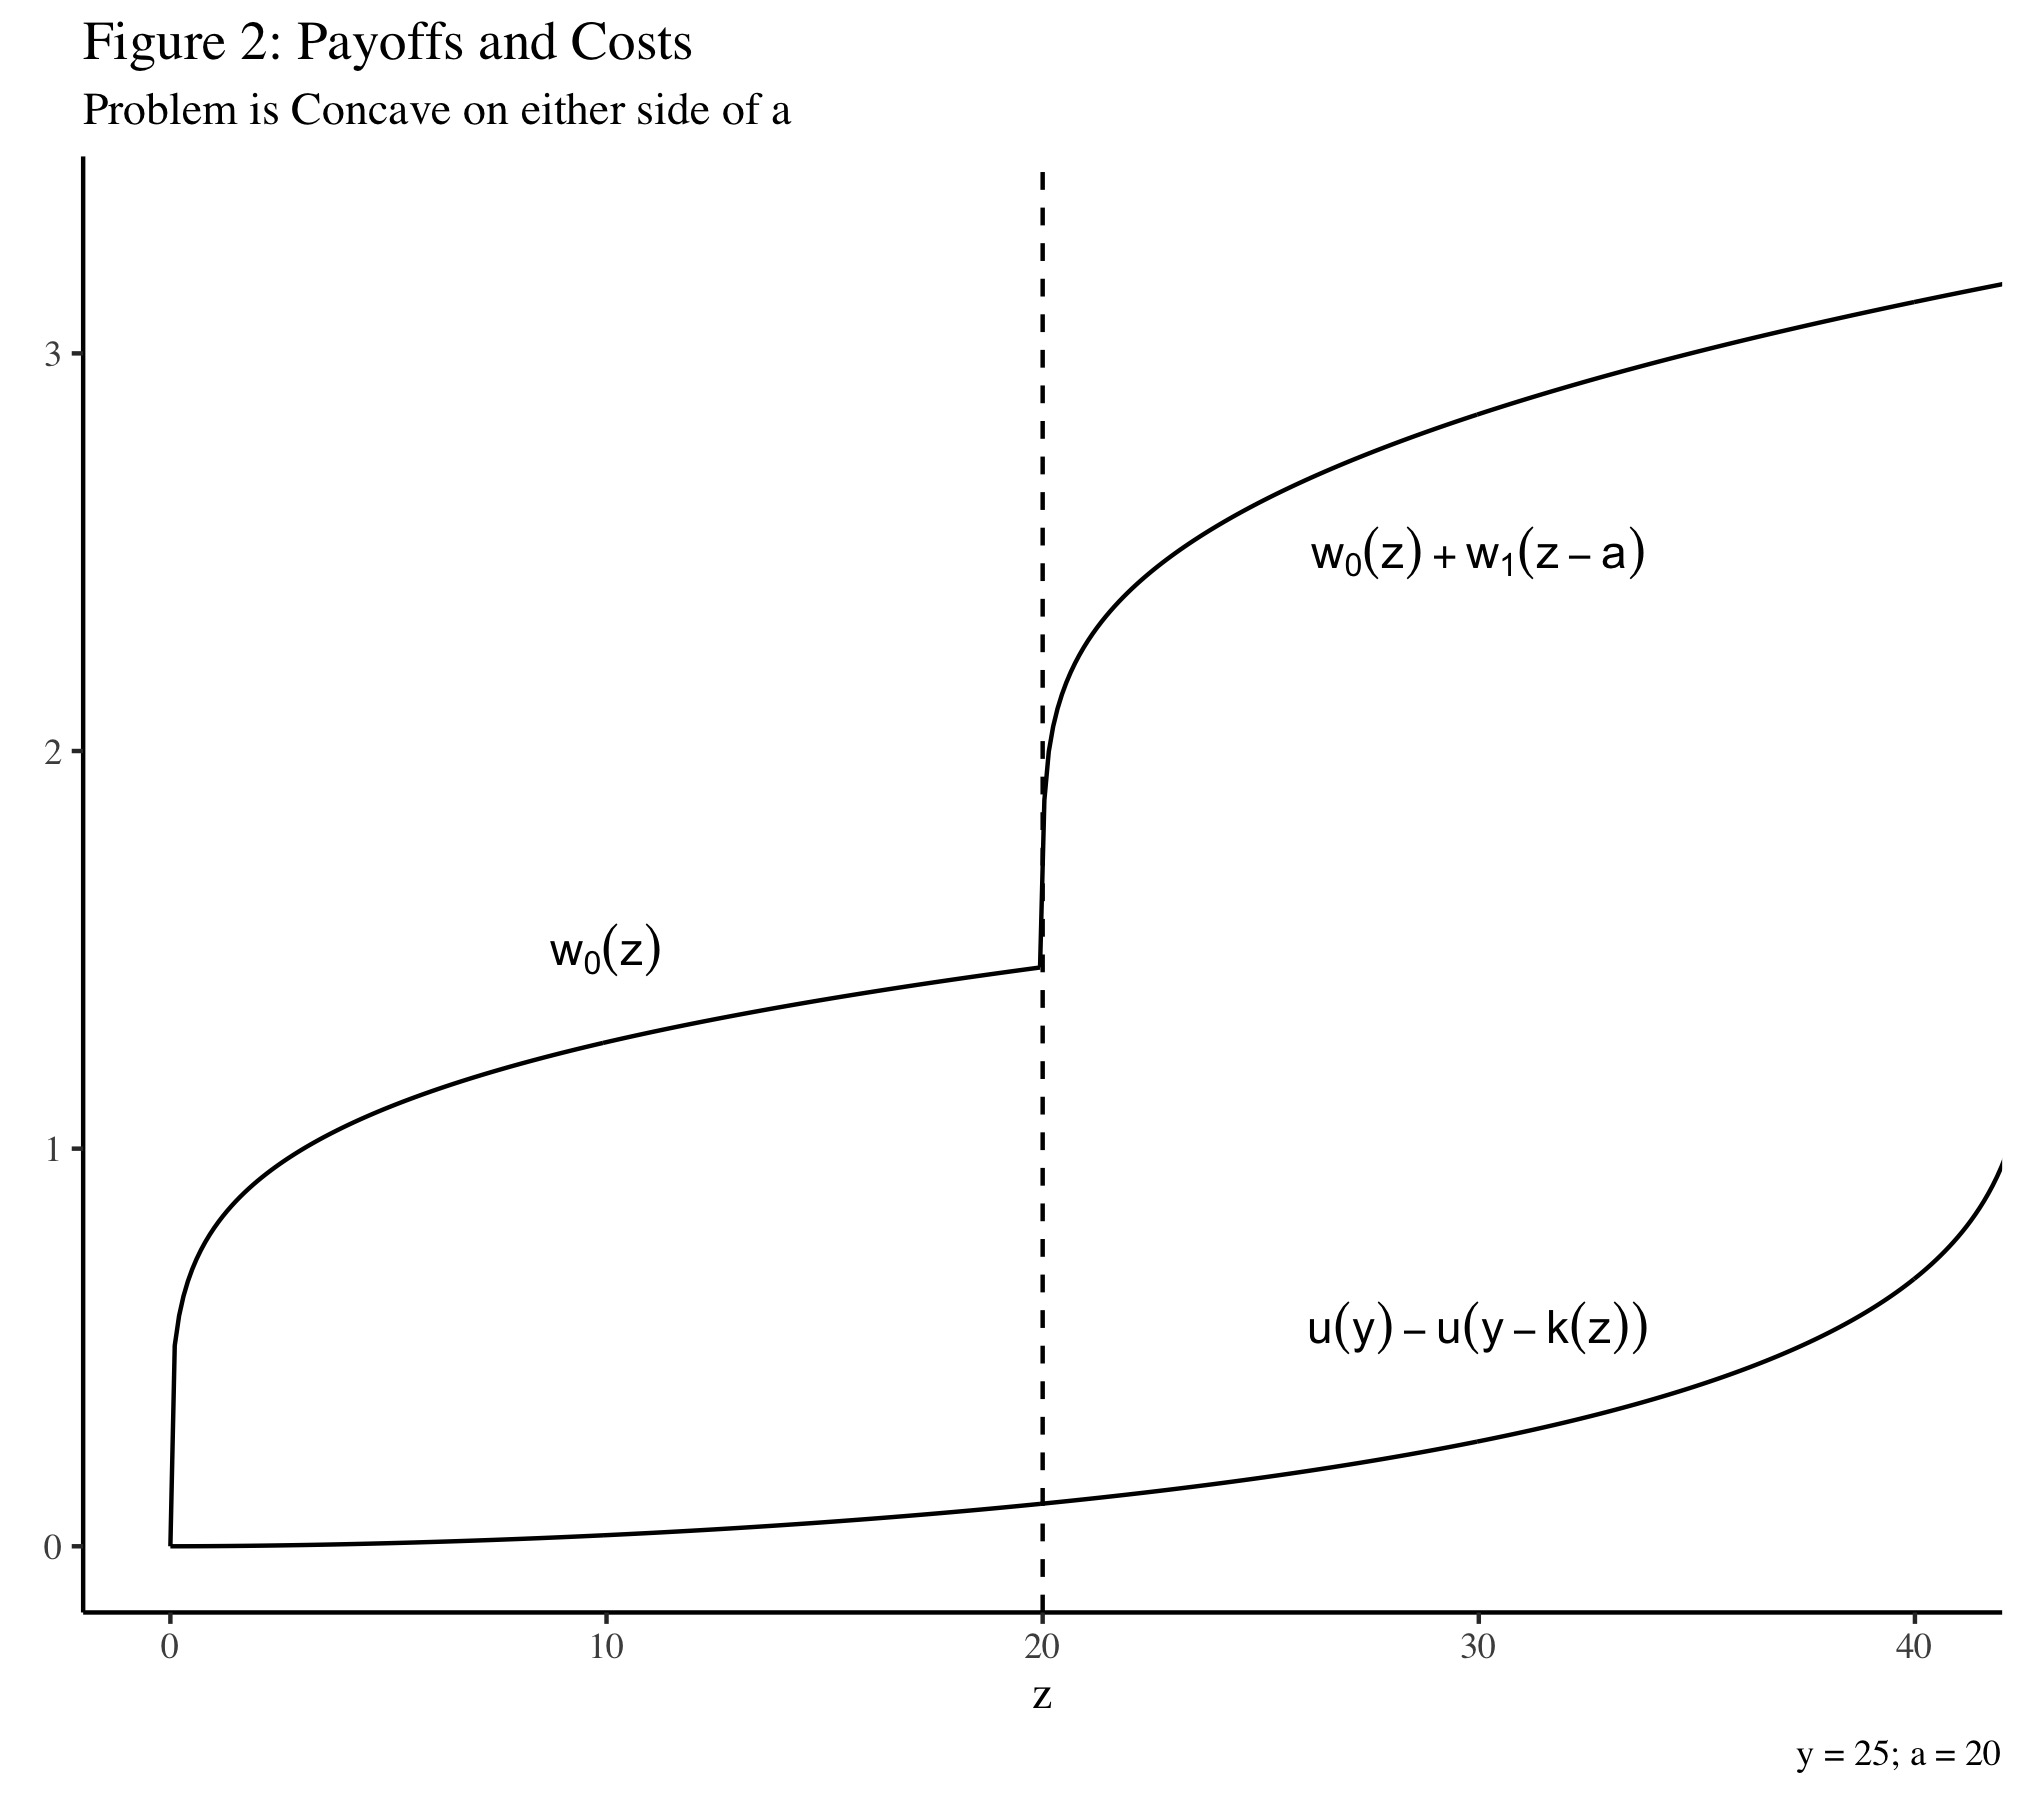
\includegraphics[scale = 0.15]{figures/fig2.jpg}
    \end{figure}
    Here, the upper curves showing \( w_0(z) + w_1(\max\{z - a, 0\}) \) illustrate the benefit of bequest \( z \) relative to aspiration \( a \), while the lower curve \( u(y) - u\left( y - k(z) \right) \) illustrates the cost. The objective of the parent is to maximize the distance between these curves. This chart illustrates that for every \( a \), the parent's problem is concave on either side of \( a \). Thus, the parent has at most two first-order conditions to solve: for \( z > a \), 
    \begin{equation}
        w_0^\prime(z) + w_1^\prime(z - a) = \frac{u^\prime(y - k(z))}{f^\prime(k(z))} \label{zopt0}  
    \end{equation}
    and for \( z < a \), 
    \begin{equation}
        w_0^\prime(z) = \frac{u^\prime(y - k(z))}{f^\prime(k(z))} \label{zopt1}
    \end{equation}
    Note that the maximum feasible value for \( z \) is equal to \( f(y) \), and occurs if \( c = 0 \). Thus, if \( a < f(y) \), the aspiration can be feasibly satisfied (even if it is not optimal), and thus the parent considers the values of \( z \) that solve (\ref{zopt0}) and (\ref{zopt1}), and chooses the \( z \) with a higher payoff. If, on the other hand, \( a > f(y) \), the parent's aspiration will be frustrated regardless of their choice of \( k \), and thus they will choose the value of \( z \) which solves (\ref{zopt0}). 
    % Threshold a
    Thus, for a given value of \( y \), the authors show that up to a given level of aspiration \( a^* \), parents will select \( z_1 \) solving (\ref{zopt1}), which will increase with \( y \). These parents will have aspirations that are \textit{satisfied}. Above \( a^* \),meanwhile, the parents will select a constant \( z_0 \), which is insensitive to their aspiration \( a \). These parents' aspirations will be \textit{frustrated}. 
    \section{Growth}
    % Constant elasticity growth model
    \subsection{Constant Elasticity Growth Model}
    In order to illustrate the effect of aspirations on income growth and inequality, the authors introduce the \textit{constant elasicity growth model}, which is parametrized as follows:
    \begin{align*}
        u(c) &= c^{1 - \sigma} & w_0(z) &= \delta z^{1 - \sigma} & w_1(e) &= \delta \pi e^{1 - \sigma}
    \end{align*}
    with curvature parameter \( \sigma = 0.8 \), discount factor \( \delta = 0.8 \), excess child wealth \( e = \max\{z - a, 0\} \), and threshold payoff \( \pi > 0 \). The benefit of this setup is that all differences in income growth will come from aspirations \( a \). To derive the growth rate, begin with the parent's problem:
    \[\max_z \left(y - \frac{z}{\rho}\right)^{1 - \sigma} + \delta\left[z^{1 - \sigma} + \pi \left(\max\{z - a, 0\}\right)^{1 - \sigma}\right]\]
    Equivalently, define the growth rate \( g\equiv z / y \), and the \textit{aspirations ratio} \( r\equiv a / y \), and the problem becomes 
    \[\max_g \left(1 - \frac{g}{\rho}\right)^{1 - \sigma} + \delta\left[g^{1 - \sigma} + \pi \left(\max\{g - r, 0\}\right)^{1 - \sigma}\right]\]
    Once again, the parents have at most two first-order conditions to solve. First, if \( g > r \), the parents select \( g(r) \) to solve 
    \[\left(1 - \frac{g(r)}{\rho}\right)^{- \sigma} = \delta\rho\left[g(r)^{- \sigma} + \pi \left(g(r) - r\right)^{-\sigma}\right]\]
    Meanwhile \( \underline{g} \) solves
    \[\left(1 - \frac{\underline{g}}{\rho}\right)^{-\sigma} = \delta\rho \underline{g}^{-\sigma} \]
    % Threshold r
    % Threshold y
    The result is similar to the static case: up to a threshold aspirations ratio \( r^* \), aspirations will be \textit{frustrated}, and the parents will choose \( \underline{g} \) irrespective of \( a \). Above \( r^* \), meanwhile, they will choose \( g(r) \), which decreases in \( r \) but asymptotically approaches a growth rate above \( \underline{g} \) (\( \lim_{r\to\infty} g(r) > \underline{g} \)): 
    The authors note that given an aspirations function \( \Psi \) that exhibits social monotonicity and scale invariance, 
    \[r(y) = \frac{\Psi(y, F(y))}{y}\]
    will be decreasing in \( y \) for all \( y \). Thus, there will be a unique threshold \( y^* \) corresponding to \( r^* \) above which aspirations will be satisfied, and below which they will be frustrated:
    % Figure
    \begin{figure}[!ht]
        \centering
        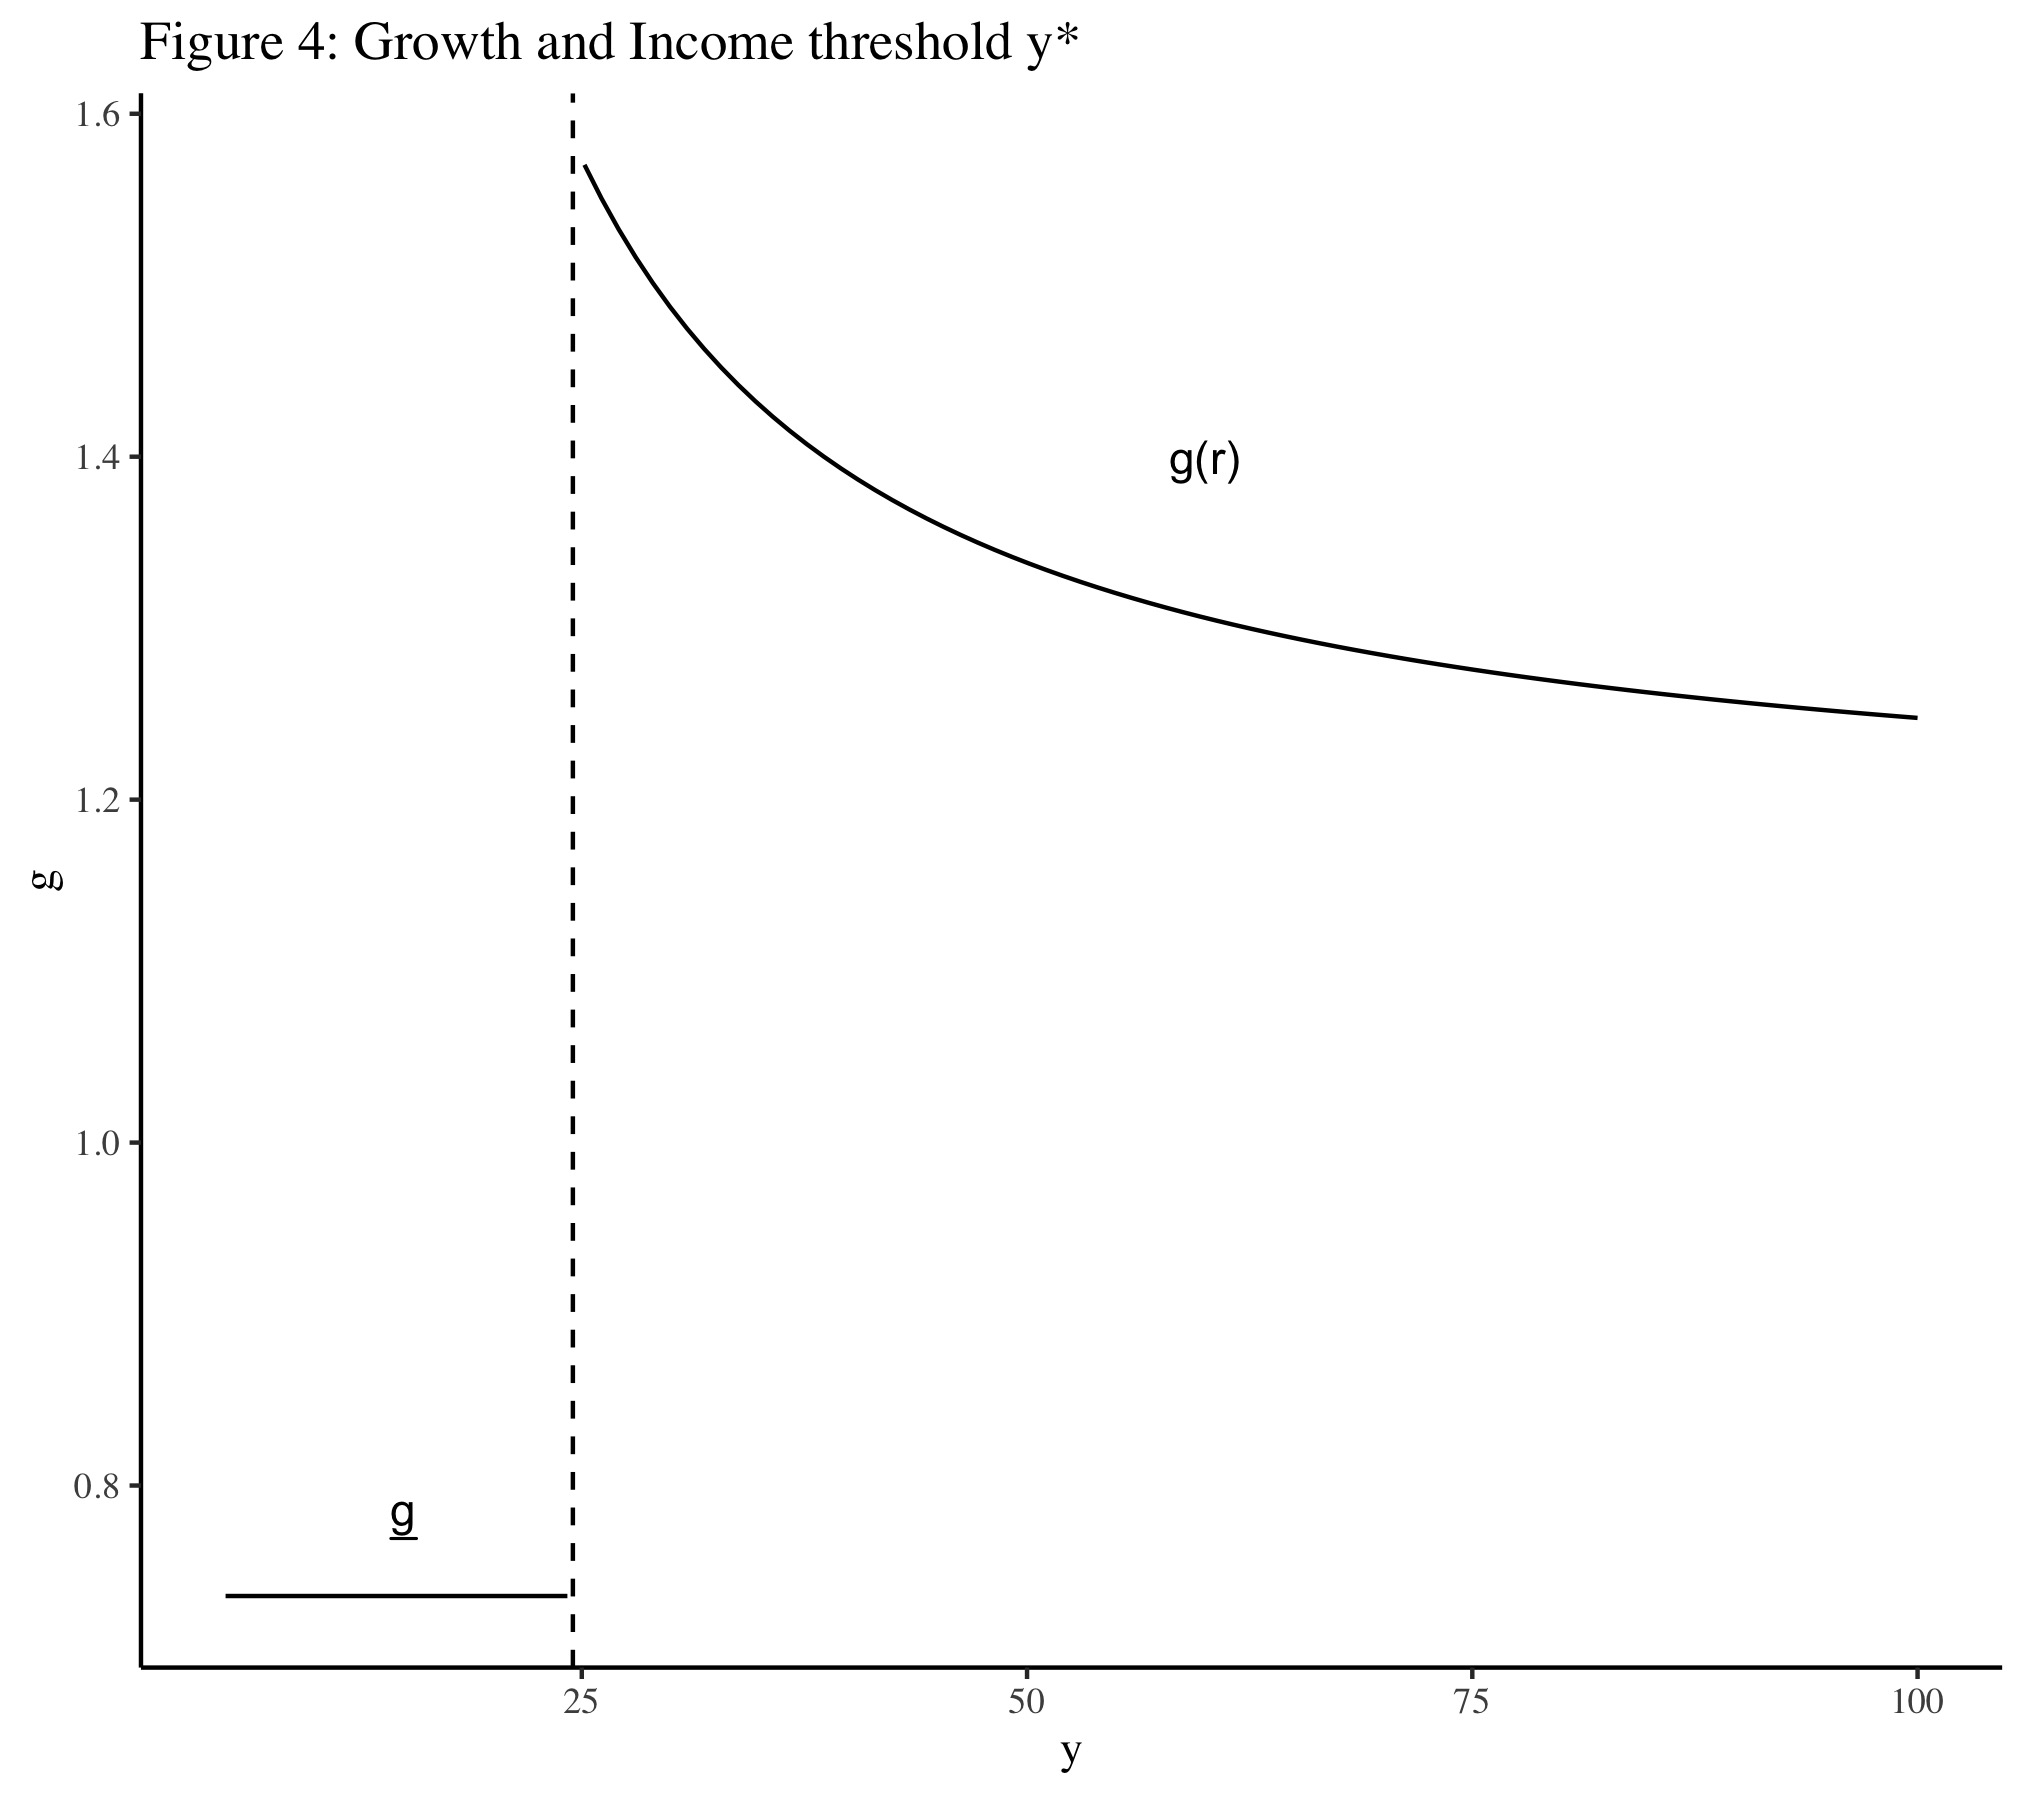
\includegraphics[scale = 0.14]{figures/fig4.jpg}
    \end{figure}
    \newpage
    As a result, in the constant-elasicity growth model, the incomes of the ``frustrated poor'' will grow at a lower rate than those of the ``satisfied rich,'' leading to forever-increasing inequality. 
    \section{Joint Evolution of Aspirations and Income}

    When discussing the evolution of incomes and aspirations, the authors make a distinction between a \textit{steady} state, and a \textit{stationary} state. A stationary state is a distribution \( F^* \) over wealth \( y \) such that each dynasty replicates itself exactly. The distinction from the steady state is that in the stationary state, the ordering of dynasties remains constant across generations; in the steady state the distribution remains constant, but the ordering of dynasties within it is allowed to change. 
    \subsection{Bounded Incomes}
    The authors begin with an example in which incomes are bounded. In order to impose such a bound, they define a new production function for bequests,
    \[f(k) = \frac{A}{\beta}k^\beta\]
    with \( A = 4 \) and \( \beta = 0.55 \), which ensures that \( f(k) < k \) for \( k \) sufficiently large. The remaining parameters are the same as in the constant-elasicity growth model. They then find a steady state distribution \( F \) by simulating the model until convergence. In this case, the authors note that no steady state can involve perfect inequality: if all incomes converve to one level, then so too will the aspirations. However, the payoff structure makes the marginal utility of accumulation above this common threshold high, and thus the system pushes away from the single income level. In this setup, a steady-state income distribution will instead be bimodal, and characterized by \( (y_\ell, y_h, p) \), where \( y_\ell \) is the low income level, \( y_h \) the high income level, and \( p \) the proportion of the population at \( y_\ell \). The following chart replicates figure 5 in the paper, which illustrates the relationship between \( y_\ell \), \( y_h \), and \( p \):
    % Figure: different values of p
    \begin{figure}[!ht]
        \centering
        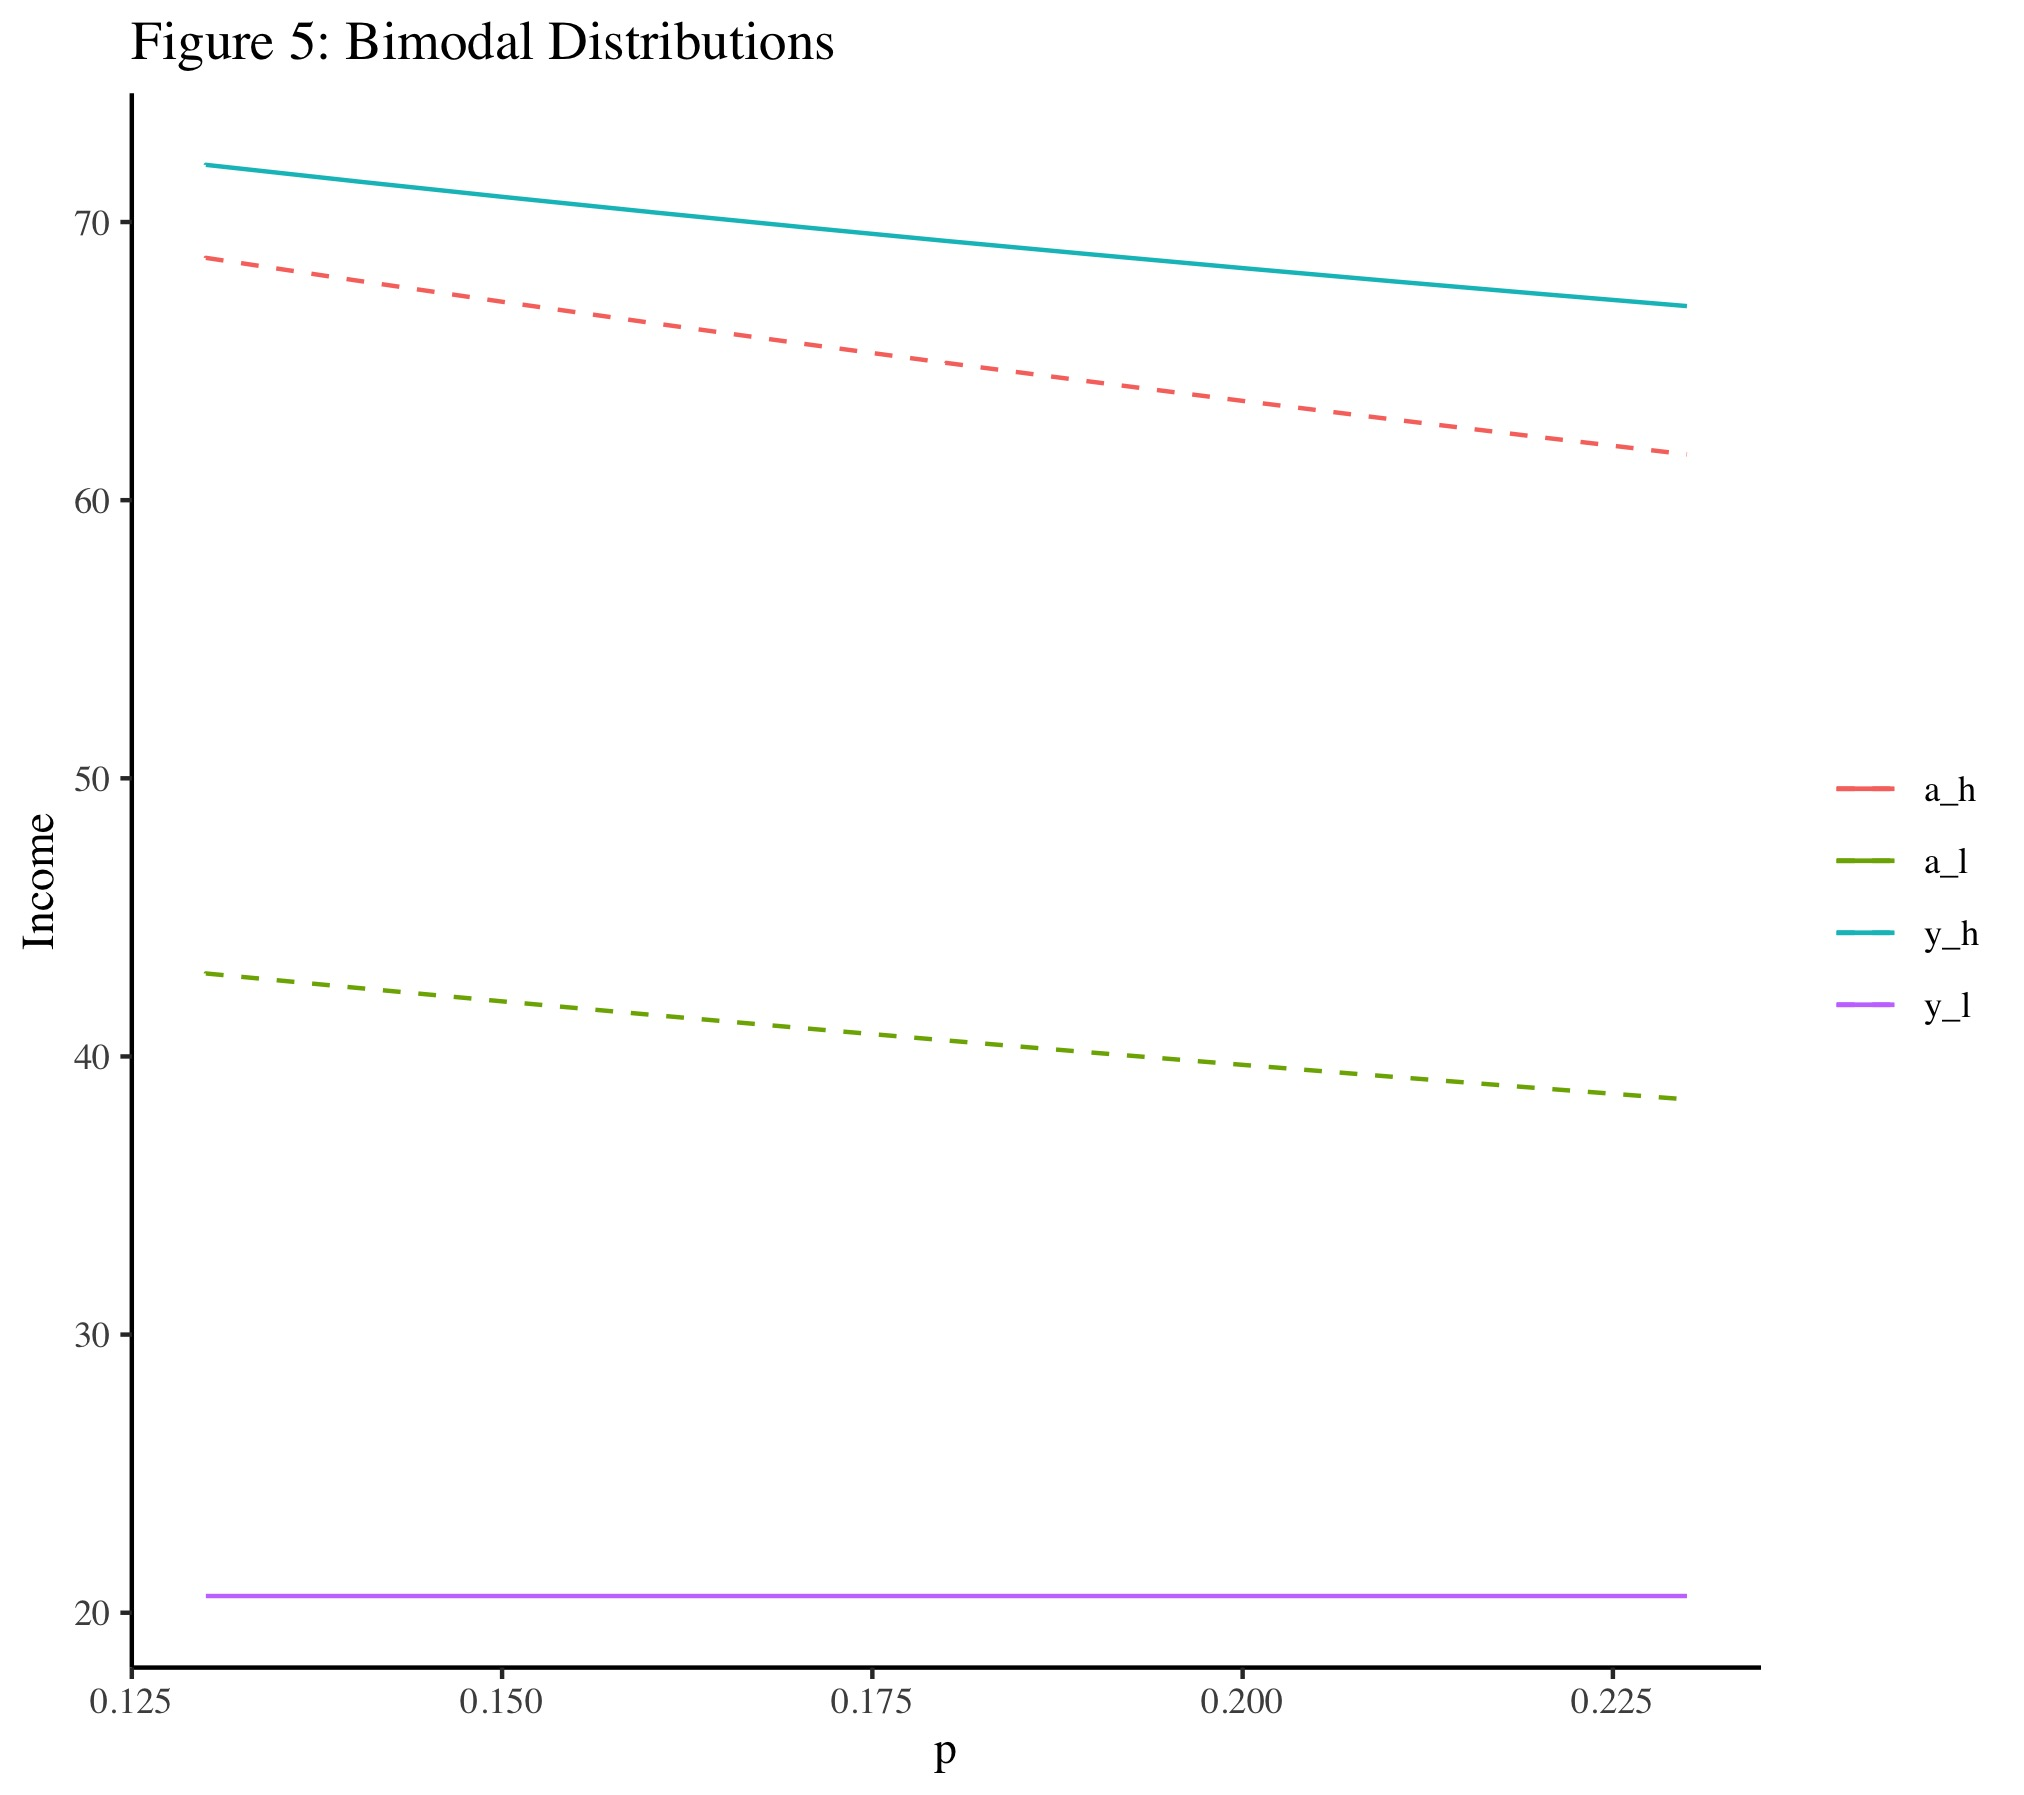
\includegraphics[scale = 0.14]{figures/fig5.jpg}
    \end{figure}
    \newpage
    In the figure above, \( a\_h \) is the aspirations of the high earners, while \( a\_l \) is the aspirations of the low earners. Also note that the distribution need not be completely degenerate: with stochasic shocks to the production function, the distribution will be smooth, and still bimodal (see Figure 6 in the paper\footnote{I am in the process of replicating this figure.}). 

    \subsection{Endogeneous Growth and Inequality}
    In a model that allows for endogeneous growth, the steady-state distribution depends on the initial distribution \( F_0 \). To illustrate this relationship, the authors return to the constant-elasticity growth model, where production is linear in bequests. Recall that agents in this parametrization choose between \( g(r) \) and \( \underline{g} \), where \( r\equiv a/y \) is the aspirations ratio. There are two possibilities:
    \begin{enumerate}
        \item Convergence to perfect equality: all incomes grow asymptotically at \( g(1) \), and normalized incomes \( y_t / g(1)^t \) converge to a single level.
        \item Persistent divergence: income growth separates into high (\( \bar{g} \)) and low (\( \underline{g} \)) levels, and normalized incomes in these groups converge. Thus, inequality is forever increasing.
    \end{enumerate}
    Which of these states occurs depends on the initial distribution \( F_0 \): if \( F_0 \) exhibits relative equality, incomes will converge (option 1). If \( F_0 \) is relatively unequal, option 2 will occur, and inequality will grow without bound. Also note that \( \underline{g} \leq \bar{g} \leq g(1) \); total growth is higher under convergence. 

    \subsection{Cognitive Windows}
    The authors allow for the possibility that individuals may only observe subsets of the distribution \( F \) when forming their aspirations, rather than the entire distribution. As an example, consider ``upper mean'' aspirations, where
    \[\Psi(y, F(y)) = \mathbb{E}_F(x | x > y)\]
    that is, individuals form their aspirations based only on incomes greater than theirs. As the authors note, this aspirations function violates the social monotonicity assumption (Figure 8). As proof, recall the observation that the aspirations ratio \( r \) is decreasing in \( y \) under social monotonicity and scale invariance. However, as seen in Figure 8, a small change in \( y \) can lead to a large increase in \( r \) using upper mean aspirations, as the increase in \( y \) moves a large mass of low incomes out of the cognitive window. Because upper mean aspirations are scale-invariant, it must be that they are not socially monotone. % want to insert figure 8
    \subsection{Relaxing Social Monotonicity Assumption}
    % TODO: finish this section
    % Example 5: balanced growth with non-degenerate distribution
    % Example 6: balanced growth with income mobility
    The authors present two examples of aspirations functions \( \Psi \) that violate social mobility: upper mean aspirations, and ``local income windows.'' Each example leads to a potentially useful result.
    \subsubsection{Upper Mean Aspirations and Balanced Growth} 
    Using the upper mean aspirations as defined above, the authors find that balanced growth is possible if the distribution of normalized incomes \( y / (1 + g)^t \) is Pareto, with unbounded support:
    \[F\left( \frac{y}{(1 + g)^t} \right) \equiv F(w) = 1 - (A / w)^{\frac{r}{r - 1}}\]
    for all \( w \geq A \) and \( (A,r) \) such that \( r \in (1, r^*] \). In this case, the distribution of normalized incomes will be nondegenerate, and grow at rate \( g > \underline{g} \), where \( \underline{g} \) is the growth rate of frustrated agents. A steady-state distribution that is nondegenerate with balanced growth above \( \underline{g} \) is not possible with socially monotone aspirations.

    \subsubsection{Local Income Windows and Balanced Growth}
    In this example, aspirations are determined by incomes ``near'' one's own, and insensitive to incomes outside of this ``window''. Formally, for some \( \beta > 0 \), \( \Psi(y, F) \) is only a function of the support of \( F \) restricted to \( [y(1 - \beta), y(1 + \beta)] \). A result of these aspirations is that it becomes impossible for an individual to remain frustrated relative to their aspirations forever: either I cross my threshold, or the individuals near me disappear from my ``window'' and my aspirations adjust downward. 
    
    As a concrete example, the authors consider a distribution with mass at three points: \( y_1 \), \( y_2 \), and \( y_3 \), representing rich, middle-class, and poor incomes, respectively (\( y_1 > y_2 > y_3 \)). The aspirations are such that the rich at \( y_1 \) only see the rich, the middle class see the rich incomes (and are frustrated), and the poor see only the middle-class incomes (and are satisfied). The incomes of the rich will grow at some factor \( g \) (the authors assume that they are satisfied). Because the middle class is frustrated and the poor are satisfied, the incomes of the poor will grow \textit{faster} than those of the rich, leading to \textit{income crossings}. Thus, this specification generates both balanced growth and income mobility, two features seen in the data. 
    \subsubsection{``Minimally Monotone'' Aspirations}
    To formalize the results of the previous two examples, the authors weaken the assumption of \textit{socially monotone} aspirations to one of \textit{minimally monotone} aspirations. The definition is as follows: for any distribution function \( F \), let \( F_-(y) \) denote the left-hand limit at \( y \), and suppose that \( F^\prime \) weakly dominates \( F \). If \( \bar{y} \) is the highest income in \( F \), then minimal monotonicity requires that \( \Psi(y, F^\prime) \geq \Psi(y, F) \). For \( y < \bar{y} \), minimal monotonicity requires that 
    \[\Psi(y, F^\prime) \geq \Psi(y, F)\text{ if and only if }
    F^\prime_-(y) = F_-(y)\]
    This condition weakens the assumption on aspirations. Up to this point, it was required that if the new distribution \( F^\prime \) dominated the old, then aspirations had to move upwards. Now, aspirations need only adjust upwards if incomes in \( F \) that were less than \( y \) remain less than \( y \) in \( F^\prime \). This allows for the possibility that \( F^\prime \) dominates \( F \), but an individual in \( F^\prime \) could see their relative position fall relative to \( F \), and adjust their aspirations downward--even though the distribution in general has shifted up. 

    In the constant-elasticity growth model with minimally monotone aspirations, there are three possibilities for the balanced growth path (Proposition 8, p. 509):
    \begin{enumerate}
        \item Convergence to perfect equality: all incomes grow at rate \( g(1) - 1 \), normalized incomes \( y_t / g^t \) converge to a single point. 
        \item Persistent divergence: the distribution separates, with normalized incomes converging at two points with two growth rates (forever-increasing inequality)
        \item Infinite crossings: there will be ``crossings'' between income pairs at an infinite sequence of dates, wehre a crossing between \( y^1 \) and \( y^2 \) between \( t \) and \( t+1 \) is defined as \( y^1_t > y^2_t \) and \( y^1_{t+1} < y^2_{t+1} \).
    \end{enumerate}
    \section{Further Research}
    I identify a few questions going forward:
    \begin{enumerate}
        \item I need to work on formulating the value function representation of this problem. The authors note that this is ``possible but complicated;'' doing so requires parents to forecast the endogeneously determined aspirations of all of their descendents. I will look into this more.
        \item Is there support for this setup in the data? If so, how could it be measured? If I can find a value-function representation, I would be curious to know the distribution of income/wealth generated by an Aiyagari model with these preferences. 
    \end{enumerate}
\end{document}